\subsection{Chức năng phân chia công việc (Task assignment)}
    \begin{figure}[h]
        \centering
        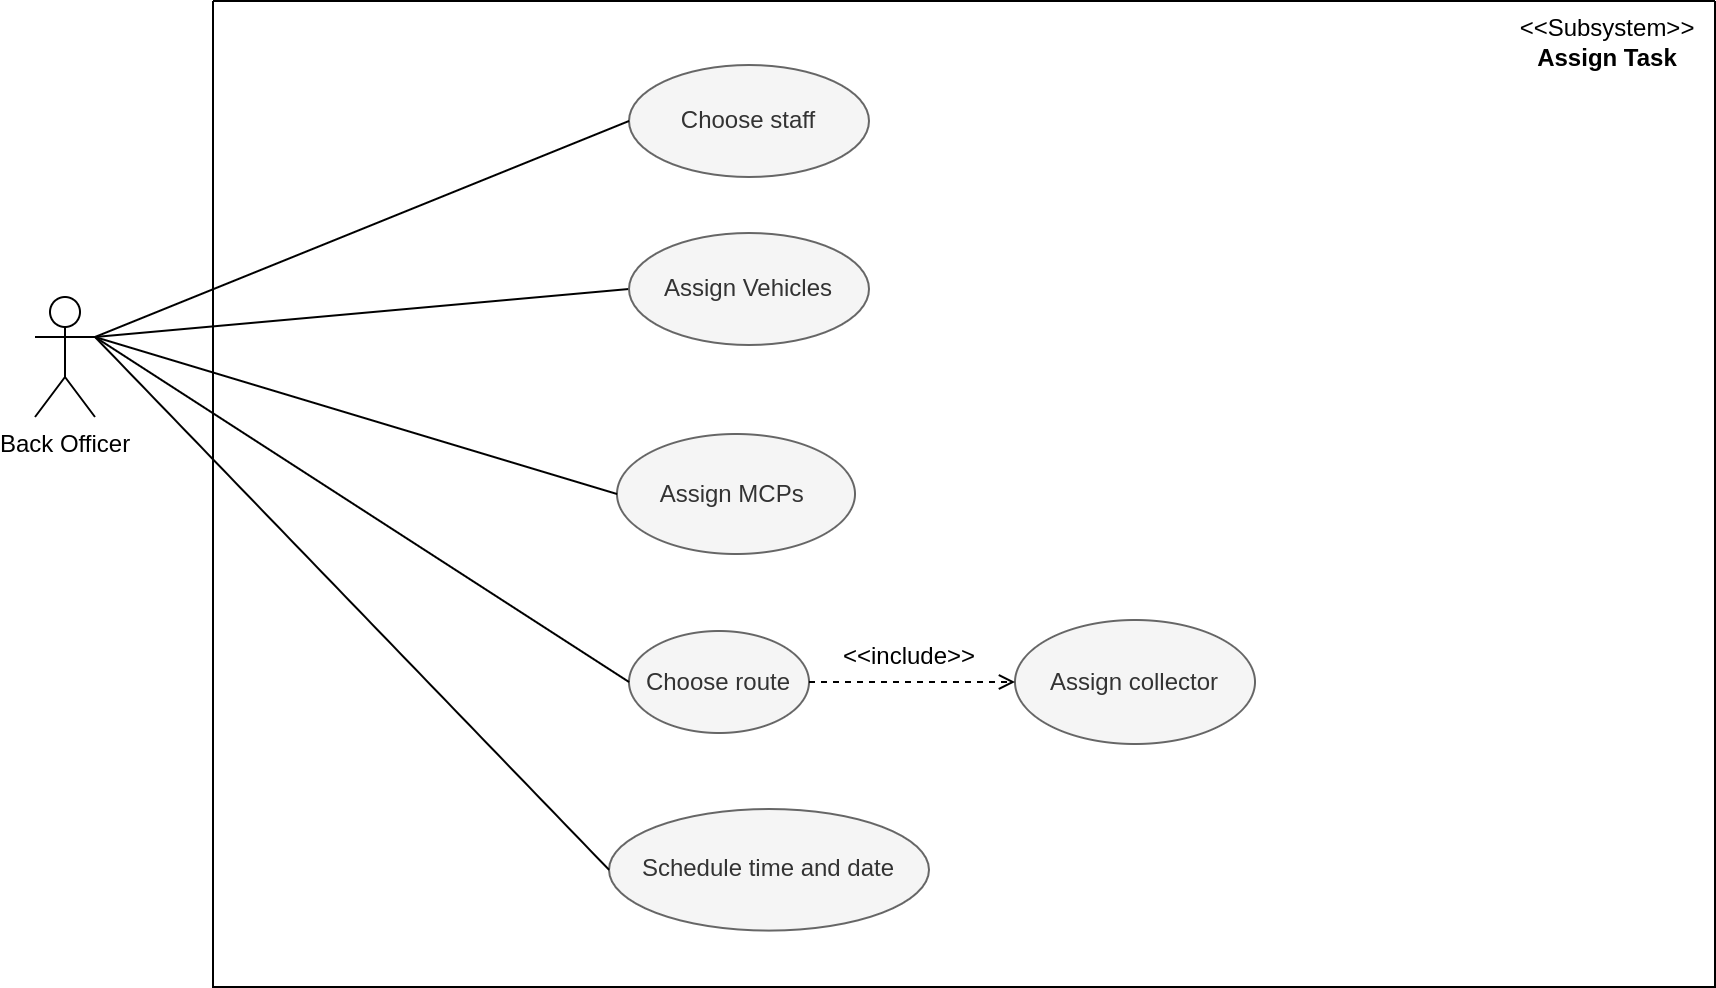
\includegraphics[width=1\linewidth]{imgs/use-case diagram/assignTask_uc.png}
        \caption{Use-case diagram chức năng phân chia công việc}
    \end{figure}
   
    \vspace{1cm}
    \begin{tblr}{
        width=1\linewidth,
        hlines,
        vlines,
        colspec={X[3]X[7]},
        columns = {valign = m, },
        row{1} = {halign = c, valign = m, bg = lightgray, fg = black},
    }
        {\textbf{Use case name} & \textbf{Choose staff}}  \\
        Description	& Chọn một nhân viên trong hệ thống \\
        Actor & 	Nhân viên giám sát (Back officer) \\
        Trigger & 		Nhân viên giám sát ấn nút chọn công nhân\\
        Pre-condition & Nhân viên giám sát đang ở phần phân công công việc \\
        Post-condition & Công nhân được chọn \\
        Normal flow &   1. Hệ thống lấy dữ liệu về công nhân \newline
                    	2. Hệ thống hiển thị các công nhân \newline
                    	3. Nhân viên giám sát chọn công nhân \newline
                    	4. Hệ thống ghi nhận công nhân được chọn \\
        Alternative flow  & none \\
        Exception flow & none \\
    \end{tblr}
  
    \begin{tblr}{
        width=1\linewidth,
        hlines,
        vlines,
        colspec={X[3]X[7]},
        columns = {valign = m, },
        row{1} = {halign = c, valign = m, bg = lightgray, fg = black},
    }
        {\textbf{Use case name} & \textbf{Choose vehicle}}  \\
        Description	& Chọn một phương tiện có trong công ty \\
        Actor & 	Nhân viên giám sát (Back officer) \\
        Trigger & 		Nhân viên giám sát ấn nút chọn công nhân\\
        Pre-condition & Nhân viên giám sát đang ở phần phân công công việc \\
        Post-condition & Phương tiện được chọn thành công \\
        Normal flow &   1. Hệ thống lấy dữ liệu về phương tiện \newline
                    	2. Hệ thống hiển thị các phương tiện \newline
                    	3. Nhân viên giám sát chọn phương tiện \newline
                    	4. Hệ thống kiểm tra phương tiện đã được lái hay chưa \newline
                    	5. Hệ thống ghi nhận phương tiện được chọn \\
        Alternative flow  & none \\
        Exception flow & Exception flow thứ 1: tại bước 4 \newline
                    	 1a. Nếu phương tiện đã được gán, thông báo cho người dùng \newline
                    	 Quay lại bước 2 \\
    \end{tblr}
  
    \vspace{1cm}
    \begin{tblr}{
        width=1\linewidth,
        hlines,
        vlines,
        colspec={X[3]X[7]},
        columns = {valign = m, },
        row{1} = {halign = c, valign = m, bg = lightgray, fg = black},
    }
        {\textbf{Use case name} & \textbf{Assign MCPs}}  \\
        Description	& Gán các điểm MCP cho công nhân \\
        Actor & 	Nhân viên giám sát (Back officer) \\
        Trigger & 	Nhân viên giám sát ấn nút chọn MCPs\\
        Pre-condition & Người quản lý đang ở phần phân công công việc \\
        Post-condition & Các điểm MCP được phân công thành công\\
        Normal flow &   1. Hệ thống lấy dữ liệu về các MCP \newline
                    	2. Hệ thống hiển thị các MCP \newline
                    	3. Nhân viên giám sát chọn MCP \newline
                    	4. Hệ thống ghi nhận các MCP được chọn \\
        Alternative flow  & Alternative flow thứ 1: tại bước 3 \newline
                        	1a. Nếu công nhân được chọn là collector, cho phép gán nhiều MCP \newline
                            \newline
                        	Alternative flow thứ 2: tại bước 3 \newline
                        	2a. Nếu công nhân được chọn là janitor, cho phép gán chỉ 1 MCP \\
        Exception flow & none \\
    \end{tblr}
  
    \begin{tblr}{
        width=1\linewidth,
        hlines,
        vlines,
        colspec={X[3]X[7]},
        columns = {valign = m, },
        row{1} = {halign = c, valign = m, bg = lightgray, fg = black},
    }
        {\textbf{Use case name} & \textbf{Choose route}}  \\
        Description	& Chọn tuyến đường cho collector \\
        Actor & 	Nhân viên giám sát (Back officer) \\
        Trigger & 	Nhân viên giám sát ấn nút chọn tuyến đường \\
        Pre-condition & Người quản lý đang ở phần phân công công việc \\
        Post-condition & Tuyến đường được chọn\\
        Normal flow &   1. Hệ thống kiểm tra công nhân được chọn là ai \newline
                    	2. Hệ thống hiển thị map trong thành phố \newline
                    	3. Hệ thống hiển thị các tuyến đường được xem là tối ưu \newline
                    	4. Nhân viên giám sát chọn tuyến đường \newline
                    	5. Hệ thống ghi nhận tuyến đường được chọn \\
        Alternative flow  & Alternative flow thứ 1: tại bước 1 \newline
                            1a. Nếu công nhân được chọn là Janitor, hệ thống thông báo và quay 	trở lại màn hình phân công công việc \\
        Exception flow & none \\
    \end{tblr}
  
    \vspace{1cm}
    \begin{tblr}{
        width=1\linewidth,
        hlines,
        vlines,
        colspec={X[3]X[7]},
        columns = {valign = m, },
        row{1} = {halign = c, valign = m, bg = lightgray, fg = black},
    }
        {\textbf{Use case name} & \textbf{Schedule time and date}}  \\
        Description	& Xếp lịch cho nhân viên \\
        Actor & 	Nhân viên giám sát (Back officer) \\
        Trigger & 	Nhân viên giám sát ấn nút set lịch làm\\
        Pre-condition & Người quản lý đang ở phần phân công công việc \\
        Post-condition & Lịch làm được phân thành công\\
        Normal flow &   1. Hệ thống lấy dữ liệu về lịch làm \newline
                    	2. Hệ thống hiển thị các ngày trong tuần \newline
                    	3. Nhân viên giám sát chọn các ca còn trống \newline
                    	4. Nhân viên xác nhận lịch đã chọn \newline
                    	5. Hệ thống ghi nhận lịch làm \\
        Alternative flow  & none \\
        Exception flow & none \\
    \end{tblr}
  
\newpage 